% !TEX encoding = UTF-8 Unicode
\documentclass[14pt]{beamer}
\usetheme{Warsaw}
\usepackage[utf8]{inputenc}

\usefonttheme{serif} % default family is serif
\usepackage[T1]{fontenc}
\usepackage{ragged2e}
\justifying
\usepackage[spanish]{babel}
\setbeamertemplate{navigation symbols}{}
\setbeamertemplate{footline}

\usepackage[absolute,overlay]{textpos}
\usepackage{anyfontsize}
\usepackage{ragged2e}
\usepackage{subfig}
\useoutertheme{split}
\justifying
\usepackage{mathtools}
\usepackage{amsmath}
\usepackage{float}
\usepackage[absolute,overlay]{textpos}
\usepackage{anyfontsize}
\usepackage{amssymb}
\usepackage{color}
\usepackage{graphicx}
\usepackage{relsize} % Para usar \mathlarger	
\usepackage{tikz}
\usepgflibrary{arrows}
\spanishdecimal{.}
\usepackage{hhline}
\usepackage{diagbox}
\usepackage{rotating}
\usepackage{xcolor}

\setbeamerfont{frametitle}{family=\fontfamily{cyklop}\selectfont \fontfamily{lmss}\selectfont} %Cambiar formato de fuente de títulos de diapositivas.



%\usepackage{caption}
%\captionsetup{font=scriptsize,labelfont=scriptsize} 
\setbeamerfont{caption}{size=\scriptsize}  

\usepackage{threeparttable}
\usepackage{caption}

\newcommand{\graficaceroeventos}[4]{
\begin{textblock*}{190mm}(-3cm,#4)
\begin{figure}[H]
%\centering
\begin{tikzpicture}
  \node{\includegraphics[scale=0.33]{#1}};
  \node at (0,3.12) {\bf {\small #2 (eje \textbf{\textit{#3}})}};
  \node at (0,-3.1) {\scriptsize Tiempo ($s$)};
  \node[black,rotate=90] at (-6,0) {\scriptsize Aceleraci{\'o}n};
\end{tikzpicture}
\end{figure}
\end{textblock*}
}

\newcommand{\graficauneventos}[4]{
\begin{textblock*}{190mm}(-3cm,#4)
\begin{figure}[H]
\begin{tikzpicture}
  \node{\includegraphics[scale=0.33]{#1}};
  \node at (0,3.12) {\bf {\small #2 (eje \textbf{\textit{#3}})}};
  \node at (0,-3.1) {\scriptsize Tiempo ($s$)};
  \node[black,rotate=90] at (-6,0) {\scriptsize Aceleraci{\'o}n};
  \node at (4.5,2.6) {\fontsize{6}{1}\selectfont Regular};
  \node at (4.48,2.35) {\fontsize{6}{1}\selectfont #2};
\end{tikzpicture}
\end{figure}
\end{textblock*}
}

\newcommand{\graficadoseventos}[5]{
\begin{textblock*}{190mm}(-3cm,#5)
\begin{figure}[H]
\centering
\begin{tikzpicture}
  \node{\includegraphics[scale=0.33]{#1}};
  \node at (0,3.12) {\bf {\small #2 (eje \textbf{\textit{#4}})}};
  \node at (0,-3.1) {\scriptsize Tiempo ($s$)};
  \node[black,rotate=90] at (-6,0) {\scriptsize Aceleraci{\'o}n};
  \node at (4.5,2.6) {\fontsize{6}{1}\selectfont Regular};
  \node at (4.5,2.35) {\fontsize{6}{1}\selectfont Zig-zag};
  \node at (4.5,2.1) {\fontsize{6}{1}\selectfont #3};
\end{tikzpicture}
\end{figure}
\end{textblock*}
}

\newcommand{\graficadeteccion}[8]{
\begin{textblock*}{190mm}(-3cm,#8)
\begin{figure}[H]
\centering
\begin{tikzpicture}
  \node{\includegraphics[scale=0.33]{#1}};
  \node at (0,3.12) {\begin{minipage}{12cm}\centering \bf \small Detecci{\'o}n en el recorrido #2 \end{minipage}};
  \node at (0,-3.1) {\scriptsize Tiempo ($s$)};
  \node[black,rotate=90] at (-6,0) {\scriptsize Evento};
  \node at (4.7,2.59) {\fontsize{6}{1}\selectfont #4};
  \node at (4.7,2.33) {\fontsize{6}{1}\selectfont #5};
  \node at (4.7,2.08) {\fontsize{6}{1}\selectfont #6};
  \node at (4.7,1.83) {\fontsize{6}{1}\selectfont #7};
\end{tikzpicture}
\end{figure}
\end{textblock*}
}

\newcommand{\graficasalidas}[7]{
\begin{textblock*}{190mm}(-3cm,#7)
\begin{figure}[H]
\centering
\begin{tikzpicture}
  \node{\includegraphics[scale=0.33]{#1}};
  \node at (0,3.12) {\begin{minipage}{11cm}\centering \bf \small Salidas en el recorrido #2 \end{minipage}};
  \node at (0,-3.1) {\scriptsize Tiempo ($s$)};
  \node[black,rotate=90] at (-6,0) {\scriptsize Valor de la salida};
  \node at (4.13,2.58) {\fontsize{6}{1}\selectfont #3};
  \node at (4.13,2.33) {\fontsize{6}{1}\selectfont #4};
  \node at (4.13,2.08) {\fontsize{6}{1}\selectfont #5};
\end{tikzpicture}
\end{figure}				
\end{textblock*}
}

\newcommand{\graficatreseventos}[7]{
\begin{textblock*}{190mm}(-3cm,#7)
\begin{figure}[H]
\centering
\begin{tikzpicture}
  \node{\includegraphics[scale=0.33]{#1}};
  \node at (0,3.12) {\bf \small {#2 (eje \textbf{\textit{#6}})}};
  \node at (0,-3.1) {\scriptsize Tiempo ($s$)};
  \node[black,rotate=90] at (-6,0) {\scriptsize Aceleraci{\'o}n};
  \node at (4.5,2.59) {\fontsize{6}{1}\selectfont Regular};
  \node at (4.5,2.35) {\fontsize{6}{1}\selectfont #3};
  \node at (4.5,2.1) {\fontsize{6}{1}\selectfont #4};
  \node at (4.5,1.85) {\fontsize{6}{1}\selectfont #5};
\end{tikzpicture}
\end{figure}
\end{textblock*}
}

\newcommand{\graficaespectros}[5]{
\begin{textblock*}{190mm}(-2.7cm,#4)
\begin{figure}[H]
\centering
\begin{tikzpicture}
  \node{\includegraphics[scale=0.33]{#1}};
  \node at (0,3.12) {\bf \small {#2 (eje \textbf{\textit{#3}})}};
  \node at (0,-3.1) {\scriptsize Frecuencia ($Hz$)};
  \node[black,rotate=90] at (-6,0) {\scriptsize Amplitud};
  \node at (3.45,2.58) {\fontsize{6}{1}\selectfont #5};
  \node at (6.55,3.18) {\fontsize{6}{1}\selectfont };
\end{tikzpicture}
\end{figure}
\end{textblock*}
}

\setbeamertemplate{caption}[numbered]
\addtobeamertemplate{navigation symbols}{}{\hspace{1em} \usebeamerfont{footline}  } %\inserttotalframenumber



\begin{document}



\title{\fontsize{17}{0}\selectfont{\fontfamily{lmss}\selectfont Estudio de la Dinámica de Conducción en \\ \vspace{.2cm} Vehículos para Determinar \\ \vspace{.1cm} Comportamientos Anómalos}}
\author[\null]{{\fontsize{12}{1}\selectfont José Alberto López López} \and \\ \vspace{.3cm} Asesor: Dr. Antonio Marín Hernández}%\inst{1}}
%\\
%\vspace{.3cm}
%Asesor: Antonio Marín Hernández}
%\institute{Universidad Veracruzana}
\vspace{-1cm}
%\subject{Seminario de investigación}


\begin{frame}
\fontsize{11pt}{1}\selectfont
\vskip 20pt

\includegraphics[scale=.35]{UV.pdf} 
\begin{minipage}[c][10pt]{8.5cm}
\begin{center}
\fontsize{15}{0}\selectfont{\rm \scshape \vspace{-1.5cm} Universidad Veracruzana} \\ \vskip 6pt \scshape \fontsize{12}{0}\selectfont Facultad de Física
\end{center}
\end{minipage}
\titlepage
\end{frame}

\addtobeamertemplate{navigation symbols}{}{\hspace{1em} \usebeamerfont{footline} \insertframenumber / 46 } %\inserttotalframenumber

\begin{frame}{Contenido}

\begin{itemize}
\item Introducción
\vskip 8pt
\item Objetivos
\vskip 8pt
%\item Trabajos Relacionados
%\vskip 8pt
\item Bases Teóricas y Dispositivos Utilizados
\vskip 8pt
\item Desarrollo Experimental
\vskip 8pt
\item Tratamiento de Datos y Resultados
\vskip 8pt
\item Conclusiones y Trabajo Futuro
\end{itemize}

\end{frame}



\begin{frame}{Introducción}

Los accidentes automovilísticos son una problemática social, la cual se ha intentado solucionar desde hace varios años.

\begin{figure}[H]
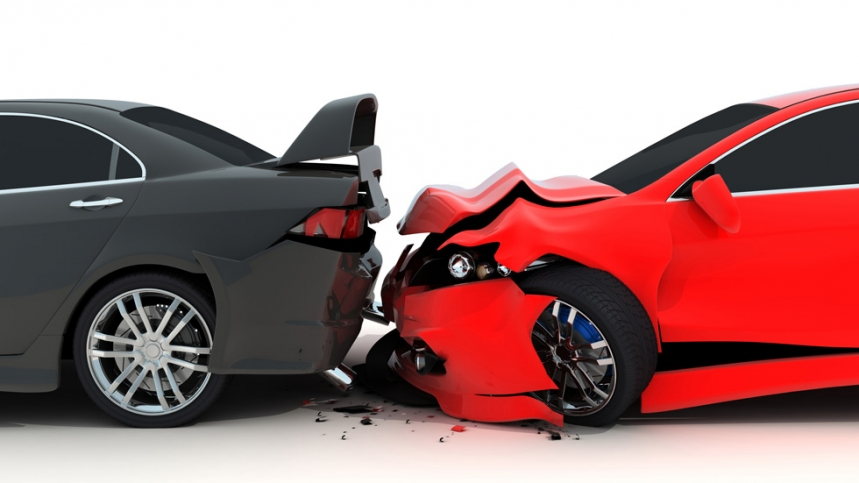
\includegraphics[scale=0.4]{choque.jpeg}
\end{figure}

\end{frame}



\begin{frame}{Introducción}

Las metodologías empleadas no siempre han sido muy eficientes.
\vspace{3.5cm}
\begin{figure}[H]
\begin{textblock*}{6cm}(1.5cm,3.7cm)
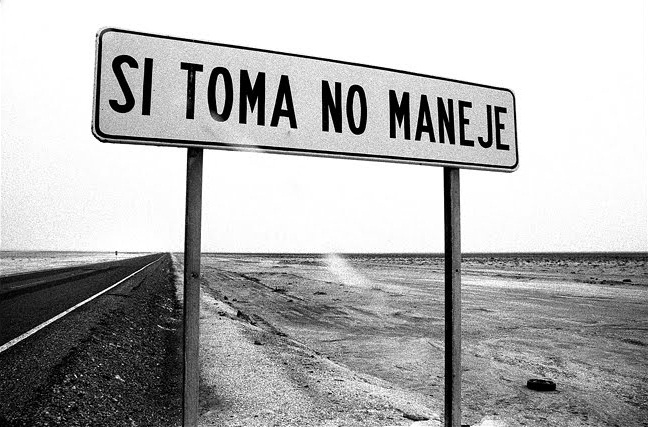
\includegraphics[scale=0.35]{senal4.jpg}
\end{textblock*}
\end{figure}
\begin{figure}[H]
\begin{textblock*}{6cm}(6.5cm,4.3cm)
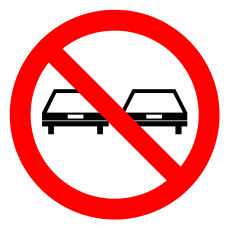
\includegraphics[scale=0.52]{senal3.png}
\end{textblock*}
\end{figure}

\end{frame}



\begin{frame}{Introducción}

Con los avances en el campo de la tecnología, es ahora posible pensar en la posibilidad de prevenir estos percances, mediante métodos de mayor eficiencia.

\begin{figure}[H]
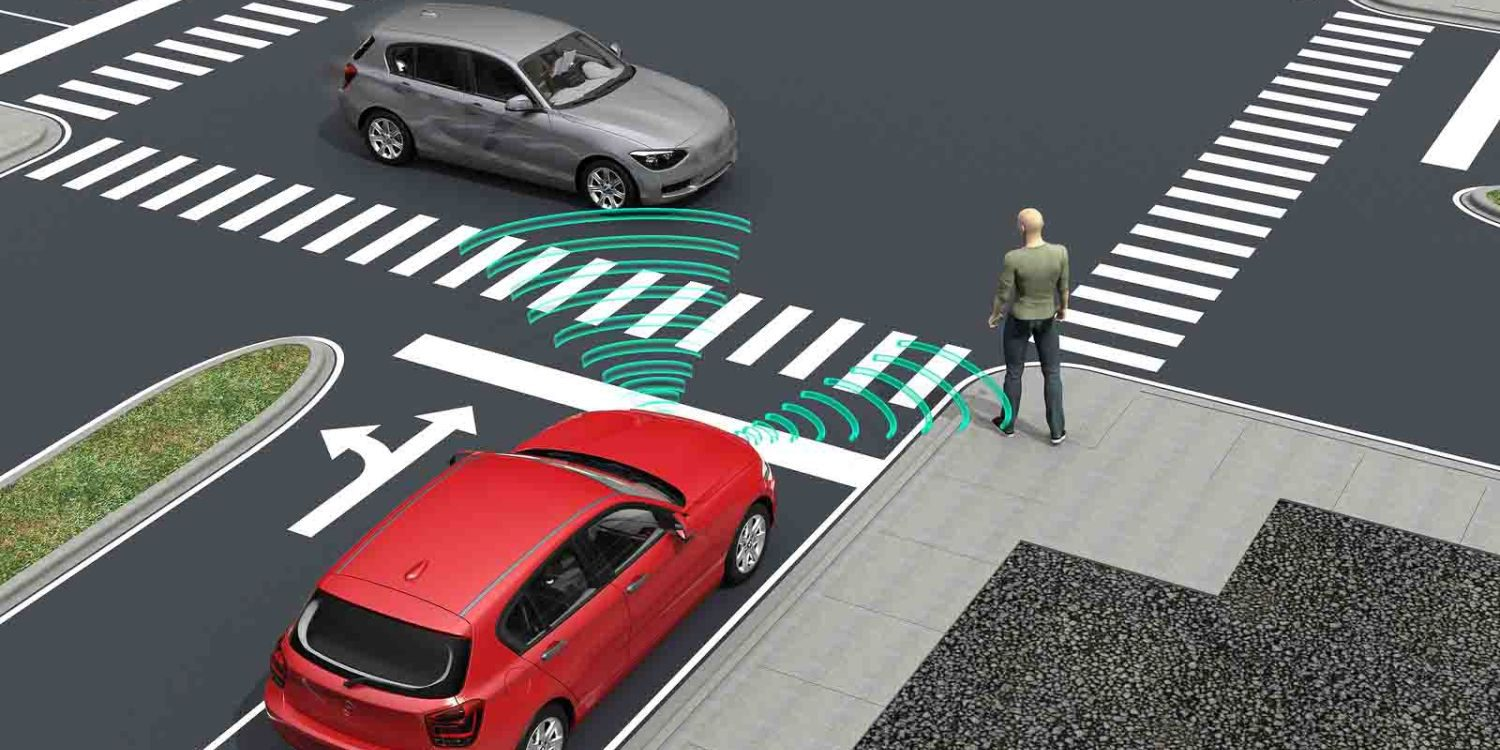
\includegraphics[scale=0.7]{autonomo.jpg}
\end{figure}

\end{frame}



\begin{frame}{Introducción}

Los proyectos hasta ahora desarrollados sobre esta temática utilizan diversas técnicas y son implementados en diferentes medios de transporte.
\vspace{5cm}
\begin{figure}[H]
\begin{textblock*}{5cm}(1cm,3.5cm)
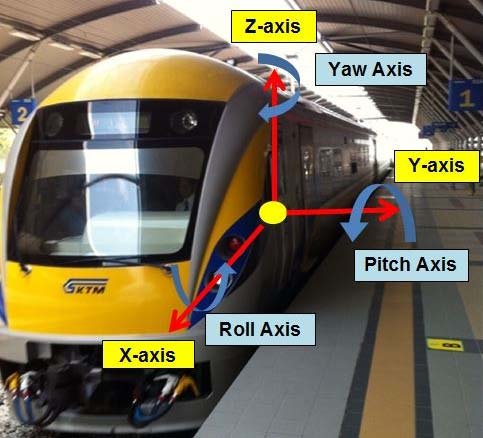
\includegraphics[scale=0.28]{4.png}
\end{textblock*}
\begin{textblock*}{5cm}(6.6cm,4.5cm)
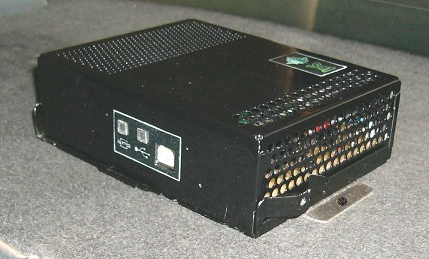
\includegraphics[scale=.4]{8.png}
\end{textblock*}
\begin{textblock*}{5cm}(1cm,7.8cm)
\caption{\justifying Sistema de ejes para el análisis de un tren. Autores: Kang Chun Hong, F. A. Hussin, y A. B. S. Saman} 
\end{textblock*}
\begin{textblock*}{5cm}(6.7cm,7.2cm)
\caption{\justifying Dispositivo para el análisis de la dinámica de un vehículo. Autores: Sylvia Noemí García Michelena y Darwin Ramiro Meneses Enríquez} 
\end{textblock*}
\end{figure}

\end{frame}



\begin{frame}{Introducción}
\begin{textblock*}{\textwidth}(1cm ,1.35cm)
%En gran parte de las investigaciones realizadas se hace uso de la tecnología integrada en los teléfonos inteligentes (figura \ref{Aplicación}), mientras que en otros casos se hace uso de dispositivos alternativos para realizar un análisis más profundo (figura \ref{Electroencefalograma}).
En otras investigaciones se hace uso tanto de las tecnologías de uso común (figura \ref{Aplicación}) como de dispositivos alternativos (figura \ref{Electroencefalograma}) para medir diferentes tipos de variables involucradas en la conducción.
\end{textblock*}
\begin{figure}[H]
\begin{textblock*}{5cm}(0.8cm,4.2cm)
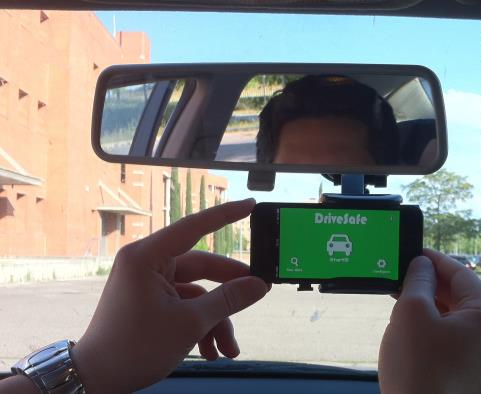
\includegraphics[scale=0.35]{App.png}
\end{textblock*}
\begin{textblock*}{5cm}(6cm,3.9cm)
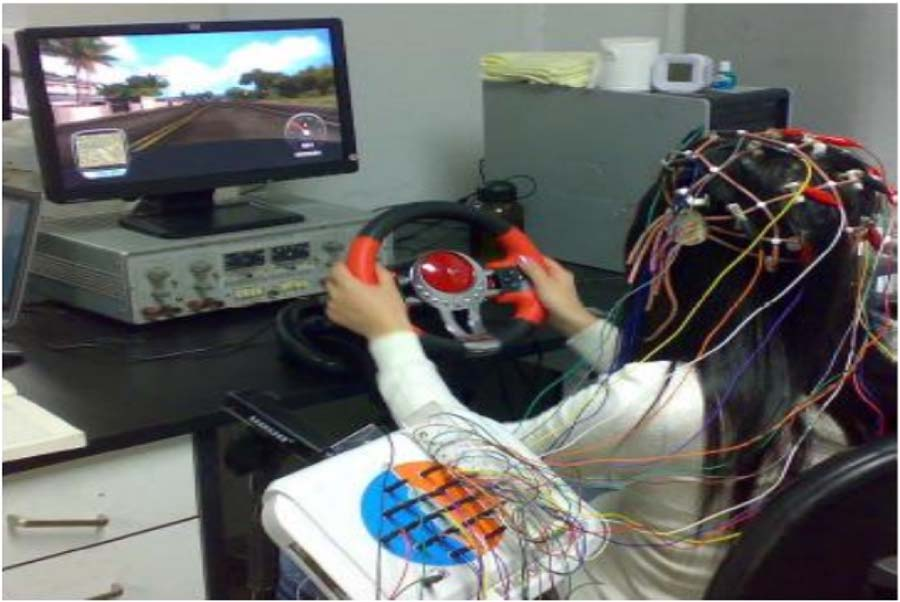
\includegraphics[scale=.2]{Electroencefalograma.png}
\end{textblock*}
\begin{textblock*}{4.7cm}(0.95cm,7.8cm)
\caption{\justifying Aplicación móvil. Autores: L. M. Bergasa, D. Almería, J. Almazán, J. J. Yebes, y R. Arroyo} 
\label{Aplicación}
\end{textblock*}
\begin{textblock*}{6cm}(6.2cm,8.1cm)
\caption{\justifying Electroencefalograma. Autores: M. V. M. Yeo, X. P. Li, K. Shen, y E. P. W. Smith} 
\label{Electroencefalograma}
\end{textblock*}
\end{figure}

\end{frame}



\begin{frame}{Introducción}

Dentro de los métodos más populares se encuentra la utilización de umbrales de aceleración y/o velocidad.

\begin{table}[H]
\centering
\begin{tabular}{|c|c|}
\multicolumn{2}{p{8cm}}{\centering \bf Event thresholds} \\ % p{ancho de texto}
\hline
\bf Event Type & \bf Threshold Sensitivity \\ 
\hline
Acceleration & $a_x > 0.1g$ \\ 
\hline
Braking & $a_x < -0.1g$ \\ 
\hline
Turn (Left) & $a_y > 0.2g$ \\
\hline
Turn (Right) & $a_y < -0.2g$ \\ 
\hline
\end{tabular}
\captionsetup{labelformat=default,font=scriptsize,margin={25pt,0pt},width=9cm,skip=10pt,justification=centering,singlelinecheck=false}
\renewcommand{\tablename}{Tabla} 
\caption{\justifying Autores: Johannes Paefgen, Flavius Kehr, Yudan Zhai, y Florian Michahelles}
\end{table}

\end{frame}



\begin{frame}{Introducción}

En el presente trabajo se pretende realizar un análisis de la dinámica de un vehículo en base a los patrones establecidos en sus datos de aceleración, con el fin de detectar movimientos anómalos; para lo cual se utilizarán los espectros de frecuencias característicos de estos datos, al analizarlos como series de tiempo.

\end{frame}



\begin{frame}{Objetivos} 

{\bf Objetivo general:\\}
\vskip 10pt
Detectar movimientos y comportamientos anómalos en trayectorias de vehículos a través del análisis de señales.\\

\end{frame}



\begin{frame}{Objetivos} 

\begin{itemize}
\item \justifying Estudiar y comprender el funcionamiento de los dispositivos a utilizar.
\item \justifying Realizar un muestreo de campo para generar una base de datos.
\item \justifying Identificar las frecuencias correspondientes al ruido (movimiento del motor) para posteriormente suprimirlas de los datos.
\item \justifying Implementar un programa de cómputo para determinar, de un conjunto de movimientos anómalos, las características de cada uno.
\item \justifying Diseñar un experimento para validar el método de detección propuesto.
\end{itemize}

\end{frame}



\begin{frame}{Bases Teóricas y Dispositivos Utilizados}

La principal teoría utilizada para cumplir los objetivos planteados fue el anális de Fourier aplicado a señales discretas.
\vspace{0cm}
$$f(t_{k})=c+ \mathlarger{\mathlarger{\sum}}_{n=1}^{N-1}\ a_{n}\cos{\left( 2\pi nt_{k}\over T\right) } + b_{n}\sin{\left( 2\pi nt_{k}\over T\right) }$$
\vspace{-0.15cm}
\small $$a_{n}={1\over N}\sum_{k=0}^{N-1} f(t_{k})\cos{\left( 2\pi nt_{k}\over T\right) }$$
\vspace{0.2cm}
$$b_{n}={1\over N}\sum_{k=0}^{N-1} f(t_{k})\sin{\left( 2\pi nt_{k}\over T\right)}$$

\end{frame}



\begin{frame}{Bases Teóricas y Dispositivos Utilizados}

La captura de datos provenientes de la dinámica del vehículo se realizó mediante un sensor de aceleración, el cual está instalado dentro del mando inalámbrico Wiimote y consta de tres ejes de medición.

\begin{figure}[H]
\begin{tikzpicture}
\centering
  \node[inner sep=0pt] (A) {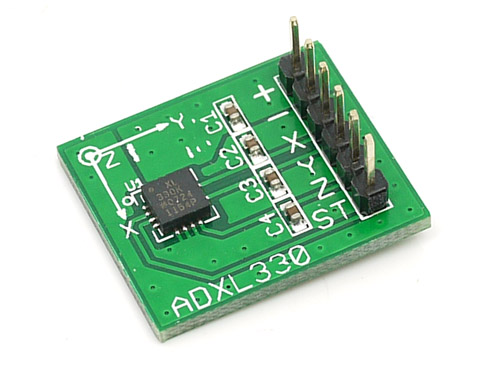
\includegraphics[scale=0.28]{adxl330v1101.jpg}\hspace{1cm}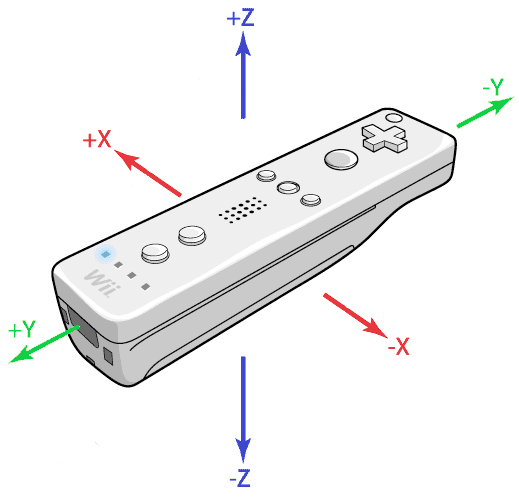
\includegraphics[scale=.28]{wiimote2.png}};
  \node at (-2,-2.4) {$a)$};
  \node at (3,-2.4) {$b)$};
%  \node at (7.7,4.1) {\small #2};
\end{tikzpicture}
\caption{$a)$ Acelerómetro. $b)$ Wiimote.}
\end{figure}

\end{frame}



\begin{frame}{Desarrollo Experimental}

Durante la etapa experimental se realizaron seis secuencias:\\
\vskip 10pt
\begin{itemize}
\item Vehículo estático
\item Conducción regular
\item {\large\bf\textcolor[rgb]{0,0,.55}{Frenado}}
\item {\large\bf\textcolor[rgb]{0,0,.55}{Rebase}}
\item {\large\bf\textcolor[rgb]{0,0,.55}{Movimiento en zig-zag}}
\item Recorrido para validación
\end{itemize}

\end{frame}



\begin{frame}{Desarrollo Experimental}

El evento de frenado consistió en detener al vehículo en aproximadamente $3s$, conduciendo a una velocidad de alrededor de $80Km/h$.

\begin{figure}[H]
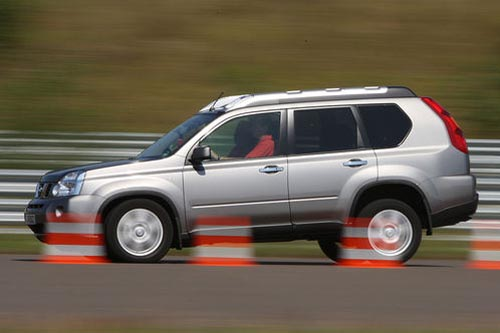
\includegraphics[scale=0.5]{Frenar.jpg}
\end{figure}

\end{frame}



\begin{frame}{Desarrollo Experimental}

El evento de rebase fue realizado ejecutando un rebase {\em común}, partiendo de una velocidad de alrededor de $80Km/h$ e incrementandola a $100Km/h$ durante el rebase.

\begin{figure}[H]
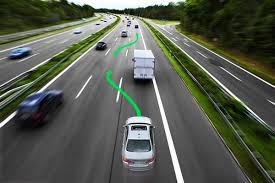
\includegraphics[scale=0.6]{Rebase.jpeg}
\end{figure}

\end{frame}



\begin{frame}{Desarrollo Experimental}

La ejecución del movimiento en zig-zag consistió en mover al vehículo de un lado a otro en repetidas ocasiones.

\begin{figure}[H]
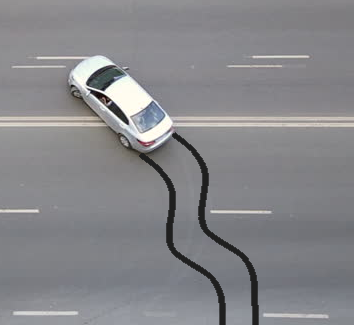
\includegraphics[scale=0.6]{Zigzag2.png}
\end{figure}

\end{frame}



\begin{frame}{Desarrollo Experimental}

Finalmente, durante el último recorrido se realizaron los tres tipos de eventos, con el fin de poner a prueba la metodología empleada para la detección.

\begin{figure}[H]
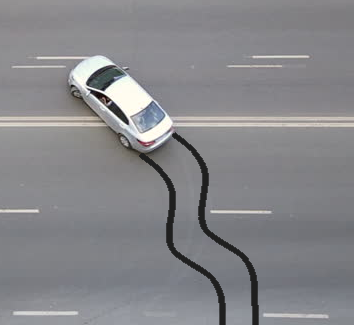
\includegraphics[scale=0.295]{Zigzag2.png} \hskip 5pt
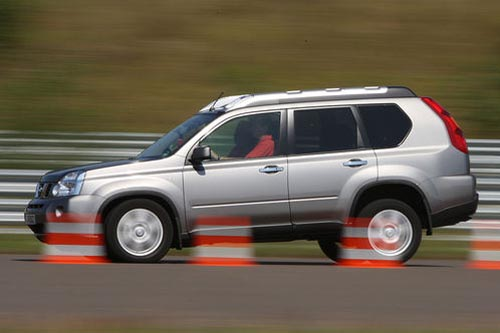
\includegraphics[scale=0.3]{Frenar.jpg} \hskip 5pt
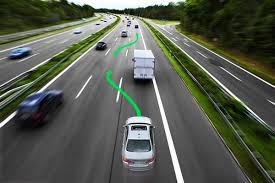
\includegraphics[scale=0.39]{Rebase.jpeg}
\end{figure}

\end{frame}



\begin{frame}{Tratamiento de Datos y Resultados}

\vspace{6.5cm}
\graficaceroeventos{1z2.pdf}{Vehículo estático}{z}{1.4cm}

\end{frame}



\begin{frame}{Tratamiento de Datos y Resultados}

\vspace{6cm}
\graficauneventos{3x.pdf}{Frenado}{x}{1.4cm}

\end{frame}



\begin{frame}{Tratamiento de Datos y Resultados}

\graficauneventos{3y.pdf}{Frenado}{y}{1.4cm}

\end{frame}



\begin{frame}{Tratamiento de Datos y Resultados}

\graficauneventos{3z.pdf}{Frenado}{z}{1.4cm}

\end{frame}



\begin{frame}{Tratamiento de Datos y Resultados}

\graficauneventos{4x.pdf}{\hskip 2pt Rebase}{x}{1.4cm}

\end{frame}



\begin{frame}{Tratamiento de Datos y Resultados}

\graficadoseventos{5y.pdf}{Movimiento en zig-zag}{Rebase}{y}{1.4cm}

\end{frame}



\begin{frame}{Tratamiento de Datos y Resultados}

\graficatreseventos{6x.pdf}{Recorrido para validación}{\hskip 2pt Zig-zag}{Frenado}{\hskip 3pt Rebase}{x}{1.4cm}

\end{frame}



\begin{frame}{Tratamiento de Datos y Resultados}

\graficatreseventos{6y.pdf}{Recorrido para validación}{\hskip 2pt Zig-zag}{Frenado}{\hskip 3pt Rebase}{y}{1.4cm}

\end{frame}



\begin{frame}{Tratamiento de Datos y Resultados}

\begin{textblock*}{190mm}(-3cm,1.4cm)
\begin{figure}[H]
%\centering
\begin{tikzpicture}
  \node{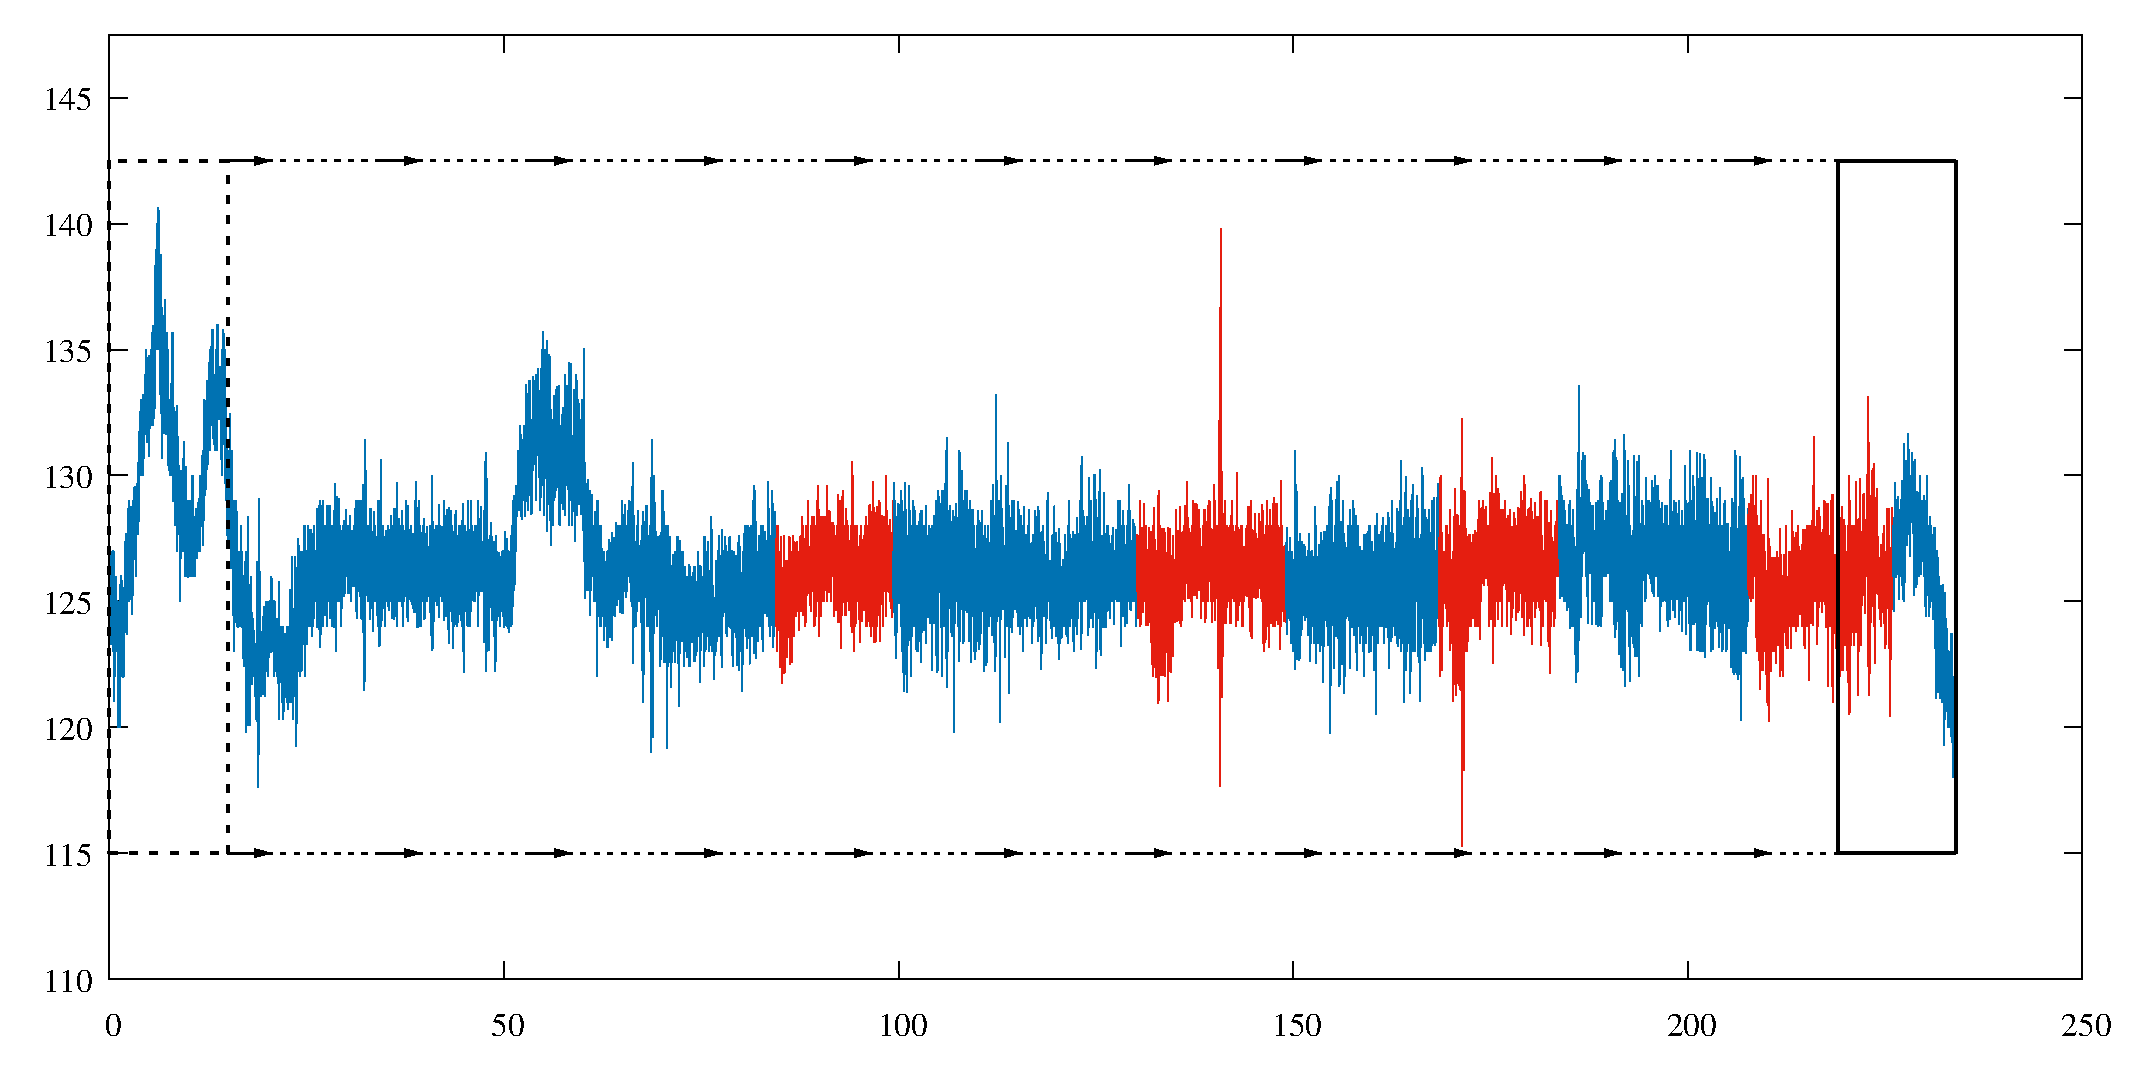
\includegraphics[scale=0.33]{Ventana.pdf}};
  \node at (0,3.12) {\bf {\small Método de detección}};
  \node at (0,-3.1) {\scriptsize Tiempo ($s$)};
  \node[black,rotate=90] at (-6,0) {\scriptsize Aceleraci{\'o}n};
\end{tikzpicture}
\end{figure}
\end{textblock*}

\end{frame}



\begin{frame}{Tratamiento de Datos y Resultados}

\begin{textblock*}{190mm}(-3cm,0.8cm)
\begin{figure}[H]
\centering
\begin{tikzpicture}
  \node{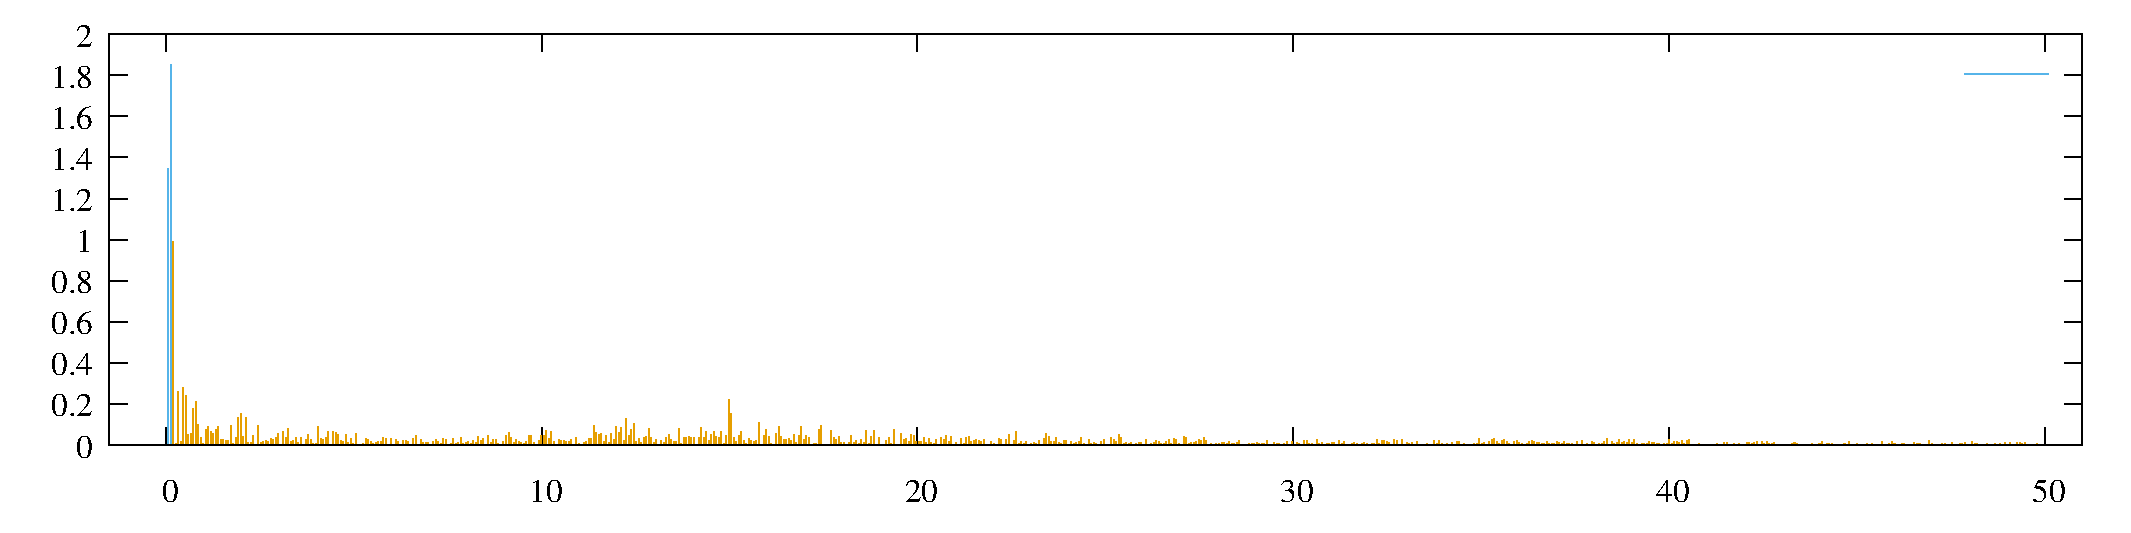
\includegraphics[scale=0.33]{Ffxs.pdf}};
  \node at (0,1.6) {\bf \footnotesize {Espectro de frecuencias (eje \textbf{\textit{x}})}};
  \node at (0,-1.6) {\scriptsize Frecuencia ($Hz$)};
  \node[black,rotate=90] at (-6,0) {\scriptsize Amplitud};
  \node at (3.45,1.1) {\fontsize{6}{1}\selectfont Frecuencias características};
\end{tikzpicture}

\vspace{0.3cm}
\begin{tikzpicture}
  \node{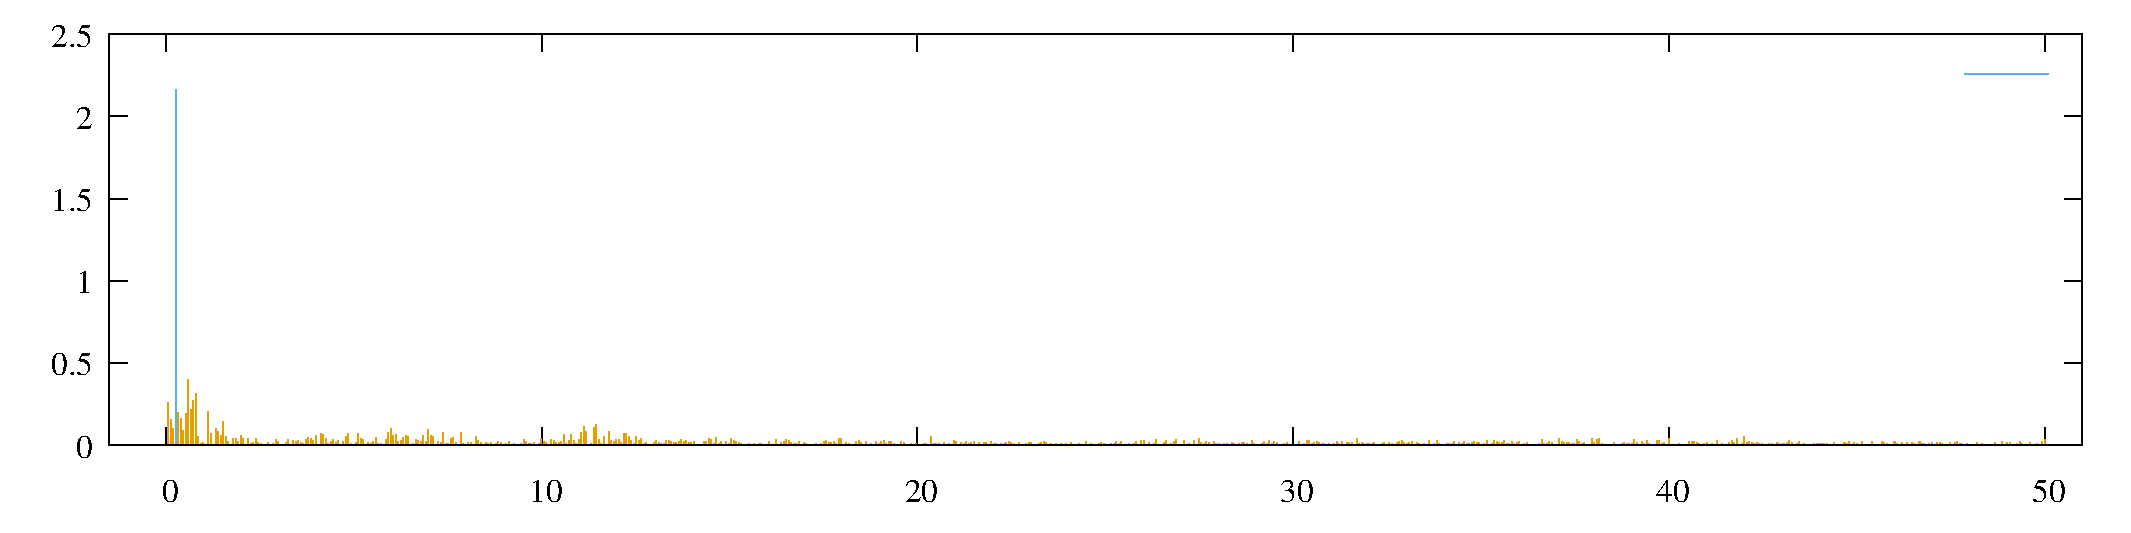
\includegraphics[scale=0.33]{Fzyc.pdf}};
  \node at (0,1.6) {\bf \footnotesize {Espectro de frecuencias (eje \textbf{\textit{y}})}};
  \node at (0,-1.6) {\scriptsize Frecuencia ($Hz$)};
  \node[black,rotate=90] at (-6,0) {\scriptsize Amplitud};
  \node at (3.56,1.1) {\fontsize{6}{1}\selectfont Frecuencia característica};
\end{tikzpicture}
\end{figure}
\end{textblock*}

\end{frame}



\begin{frame}{Tratamiento de Datos y Resultados}

\begin{figure}[H]
\centering
\vspace{8.5cm}
\begin{textblock*}{\textwidth}(-0.7cm,1.5cm)
\begin{tikzpicture}
  \node at (-8,0) {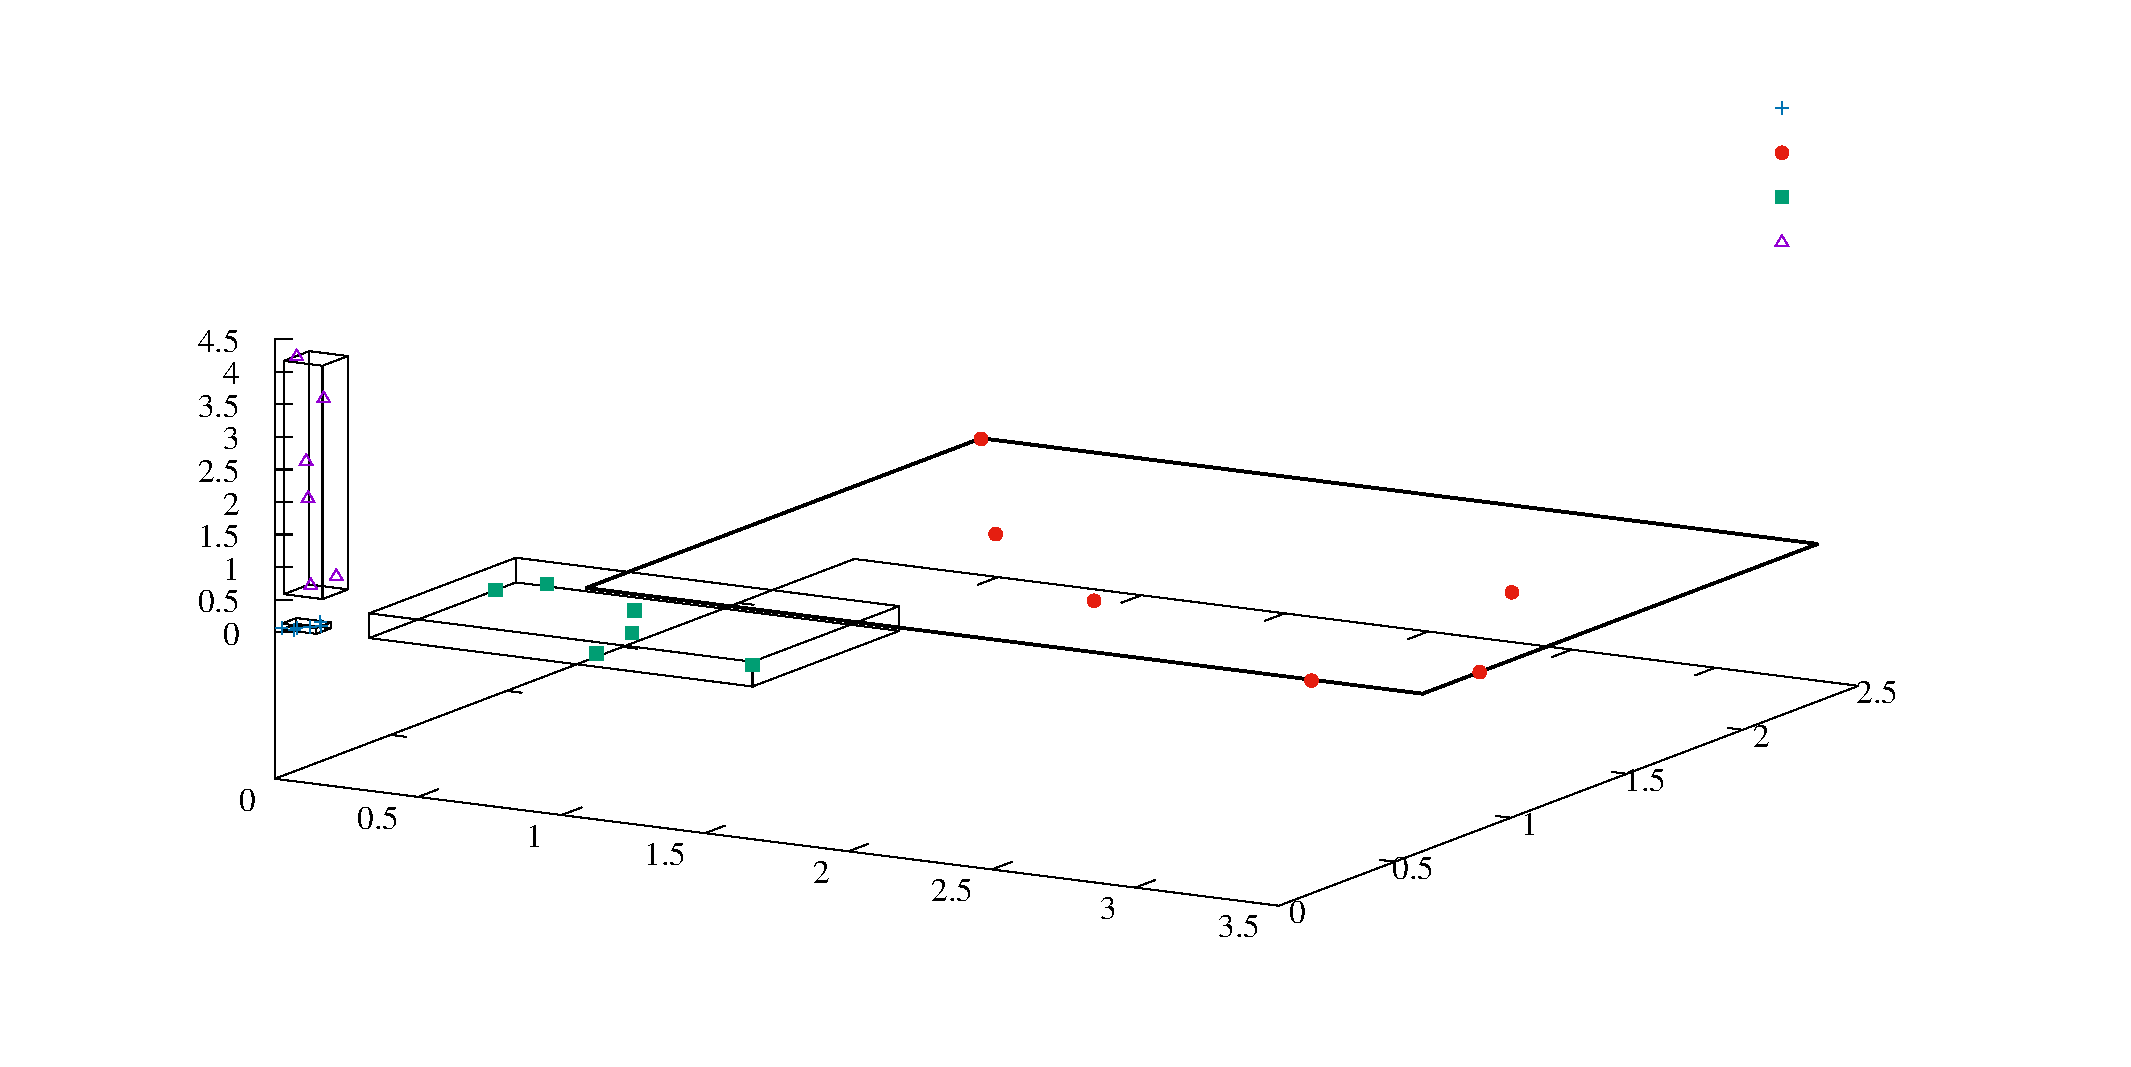
\includegraphics[scale=0.4]{Cajas.pdf}};
  \node at (-8.6,3) {\bf \small Regiones características de cada evento};
  \node[rotate=352] at (-10.4,-2.58) {\scriptsize Amplitud (0.066 Hz)};
  \node[rotate=20] at (-4.2,-2.1) {\scriptsize Amplitud (0.133 Hz)};
  \node[rotate=90] at (-14.2,0) {\scriptsize Amplitud (0.266 Hz)};
  \node at (-3.75,2.9) {\fontsize{6}{1}\selectfont Regular};
  \node at (-3.75,2.62) {\fontsize{6}{1}\selectfont Frenado};
  \node at (-3.75,2.32) {\fontsize{6}{1}\selectfont Rebase};
  \node at (-3.75,2) {\fontsize{6}{1}\selectfont Zig-zag};
\end{tikzpicture}
\end{textblock*}
\end{figure}

\end{frame}



\begin{frame}{Tratamiento de Datos y Resultados}

\begin{figure}[H]
\centering
\begin{tikzpicture}
  \node{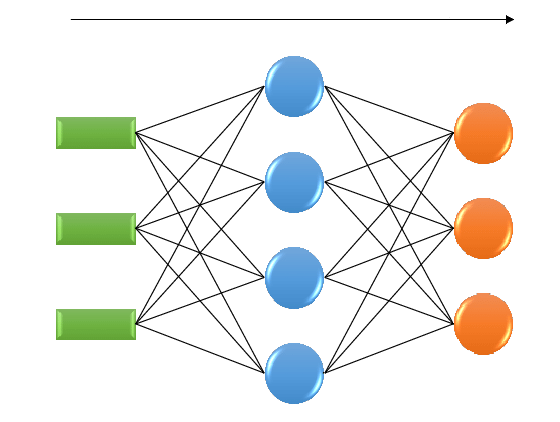
\includegraphics[scale=0.5]{Red_neuronal_2.png}};
  \node at (0,3.7) {\bf \small {Red neuronal}};
  \node at (0,2.8) {\scriptsize Información};
  \node at (-2.5,-3) {\scriptsize Capa de entrada};
  \node at (0.15,-3) {\scriptsize Capa oculta};
  \node at (2.7,-3) {\scriptsize Capa de salida};
\end{tikzpicture}
\end{figure}

\end{frame}



\begin{frame}{Tratamiento de Datos y Resultados}

\graficadeteccion{Deteccion_3_CxS.pdf}{de frenado}{}{Regular}{\hskip 2pt Rebase}{Frenado}{}{1.4cm}

\end{frame}



\begin{frame}{Tratamiento de Datos y Resultados}

\graficauneventos{3x.pdf}{Frenado}{x}{1.4cm}

\end{frame}



\begin{frame}{Tratamiento de Datos y Resultados}

\graficadeteccion{Deteccion_4_CxS.pdf}{de rebase}{}{\hskip 2pt Rebase}{Regular}{}{}{1.4cm}

\end{frame}



\begin{frame}{Tratamiento de Datos y Resultados}

\graficauneventos{4x.pdf}{\hskip 2pt Rebase}{x}{1.4cm}

\end{frame}



\begin{frame}{Tratamiento de Datos y Resultados}

\graficadeteccion{Deteccion_5_CxS.pdf}{de movimiento en zig-zag}{}{\hskip 2pt Rebase}{Regular}{\hskip 2pt Zig-zag}{}{1.4cm}

\end{frame}



\begin{frame}{Tratamiento de Datos y Resultados}

\graficadoseventos{5y.pdf}{Movimiento en zig-zag}{Rebase}{y}{1.4cm}

\end{frame}



\begin{frame}{Tratamiento de Datos y Resultados}

\graficadeteccion{Deteccion_6_CxS2.pdf}{para validación}{}{\hskip 1pt Regular}{\hskip 2pt Zig-zag}{\hskip 2.5pt Rebase}{Frenado}{1.4cm}

\end{frame}



\begin{frame}{Tratamiento de Datos y Resultados}

\graficatreseventos{6x.pdf}{Recorrido para validación}{\hskip 2pt Zig-zag}{Frenado}{\hskip 3pt Rebase}{x}{1.4cm}

\end{frame}



\begin{frame}{Tratamiento de Datos y Resultados}

\graficasalidas{Salidas_3_CxS.pdf}{de frenado}{Componente 1}{Componente 2}{Componente 3}{}{1.4cm}

\end{frame}



\begin{frame}{Tratamiento de Datos y Resultados}

\graficasalidas{Salidas_4_CxS.pdf}{de rebase}{Componente 1}{Componente 2}{Componente 3}{}{1.4cm}

\end{frame}



\begin{frame}{Tratamiento de Datos y Resultados}

\graficasalidas{Salidas_5_CxS.pdf}{de movimiento en zig-zag}{Componente 1}{Componente 2}{Componente 3}{}{1.4cm}

\end{frame}



\begin{frame}{Tratamiento de Datos y Resultados}

\graficasalidas{Salidas_6_CxS2.pdf}{para validación}{Componente 1}{Componente 2}{Componente 3}{}{1.4cm}

\end{frame}



\begin{frame}{Tratamiento de Datos y Resultados}

Los resultados obtenidos al aplicar el algoritmo de detección en el recorrido de prueba se resumen en la siguiente tabla:

\begin{table}[H]
\centering
\begin{tabular}{||c|c|c|c|c||c||}
\hhline{|t:=====:t:=:t|}
\backslashbox{\bf \small Ejecutado\\ \\ }{\\ \bf \small Detectados} & \begin{sideways}\hspace{-0.7cm}\small Regular\end{sideways} & \begin{sideways}\hspace{-0.7cm}\small Frenado\end{sideways} & \begin{sideways}\hspace{-0.7cm}\small Rebase\end{sideways} & \begin{sideways}\hspace{-0.7cm}\small Zig-zag\end{sideways} & \begin{sideways}\hspace{-0.7cm}{\bf \small Eficiencia}\end{sideways} \\ 
\hhline{||-----||-||}
\small Regular &\small 115 &\small 3 &\small 20 &\small 22 & \bf \small 0.71 \\ 
\hhline{||-----||-||}
\small Frenado &\small 5 &\small 18 &\small 0 &\small 0 & \bf \small 0.78 \\ 
\hhline{||-----||-||}
\small Rebase &\small 3 &\small 0 &\small 15 &\small 1 & \bf \small 0.78 \\ 
\hhline{||-----||-||}
\small Zig-zag &\small 0 &\small 0 &\small 0 &\small 23 & \bf \small 1 \\ 
\hhline{|b:=====:b:=:b|}
\end{tabular}
\end{table}

\end{frame}



%\begin{frame}{Conclusiones}



%\end{frame}



\begin{frame}{Conclusiones y Trabajo Futuro}

Se considera que las contribuciones más importantes, logradas del desarrollo del presente trabajo de tesis son las siguientes:
\vskip 10pt
\begin{itemize}
{\small
\item \justifying Fue posible lograr en general la detección de los tres tipos movimientos elegidos.

\item \justifying Se consiguió implementar con éxito un método poco utilizado en el ámbito del estudio de la dinámica de vehículos que determina un conjunto de características mínimas para discriminar cada evento.

\item \justifying Se determinó una combinación de las características encontradas para que por medio de una red neuronal se realizará la clasificación de los eventos.
}

\end{itemize} 

\end{frame}



\begin{frame}{Conclusiones y Trabajo Futuro}

Como continuación al trabajo presentado se propone:
\vskip 10pt
\begin{itemize}
\item \justifying Incrementar la base de datos de los eventos para mejorar la detección.
\item \justifying Aumentar el número de características discriminantes.
\item \justifying Ajustar las regiones características de cada evento (por ejemplo, convertir los prismas las a elipsoides).
\end{itemize}

\end{frame}

\begin{frame}{}
\centering
\vfill
{\fontfamily{lmss}\selectfont \Huge Gracias}
\vfill
\end{frame}

\begin{frame}{}
\begin{figure}[H]
\centering
\begin{tikzpicture}[thick]
  \node{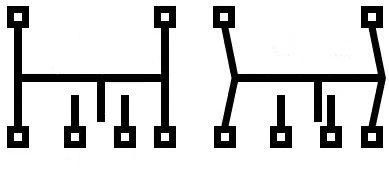
\includegraphics[scale=0.75]{mems4.jpg}};
  \node at (-3.6,1.5) {\small{\fontfamily{qhv}\selectfont Masa}};
  \node at (-2.1,1.4) {\small{\fontfamily{qhv}\selectfont Muelles}};
  \node at (3.3,1.5) {\small{\fontfamily{qhv}\selectfont Aceleración}};
  \node at (-3.6,1.1) {\small{\fontfamily{qhv}\selectfont sísmica}};
  \node at (3.3,1.1) {\small{\fontfamily{qhv}\selectfont aplicada}};
  \node at (-2.5,-2.1) {\small{\fontfamily{qhv}\selectfont Placas paralelas fijas}};
  \draw [black,-latex] (-3.6,0.85) -- (-3.6,0.55);
  \draw [black,-latex] (-1.35,1.35) -- (-0.95,1.35);
  \draw [black,-latex,line width=2pt] (2.2,1.3) -- (1.2,1.3);
  \draw [black,-latex] (-3.16,-1.9) -- (-3.16,-1.5);
  \draw [black,-latex] (-1.85,-1.9) -- (-1.85,-1.5);
\end{tikzpicture}
\end{figure}
\end{frame}



\begin{frame}{}
$$f(t)\approx c+ \sum_{n=1}^{m}\ a_{n}\cos{\left( 2\pi nt\over T\right) } + b_{n}\sin{\left( 2\pi nt\over T\right) }$$\\

$$a_{n}={2\over T}\int_{-T\over 2}^{T\over 2} f(t)\cos{\left( 2\pi nt\over T\right) }dt$$\\

$$b_{n}={2\over T}\int_{-T\over 2}^{T\over 2} f(t)\sin{\left( 2\pi nt\over T\right) }dt$$
\end{frame}



\begin{frame}{}
\begin{textblock*}{190mm}(-3.3cm,0.8cm)
\begin{figure}[H]
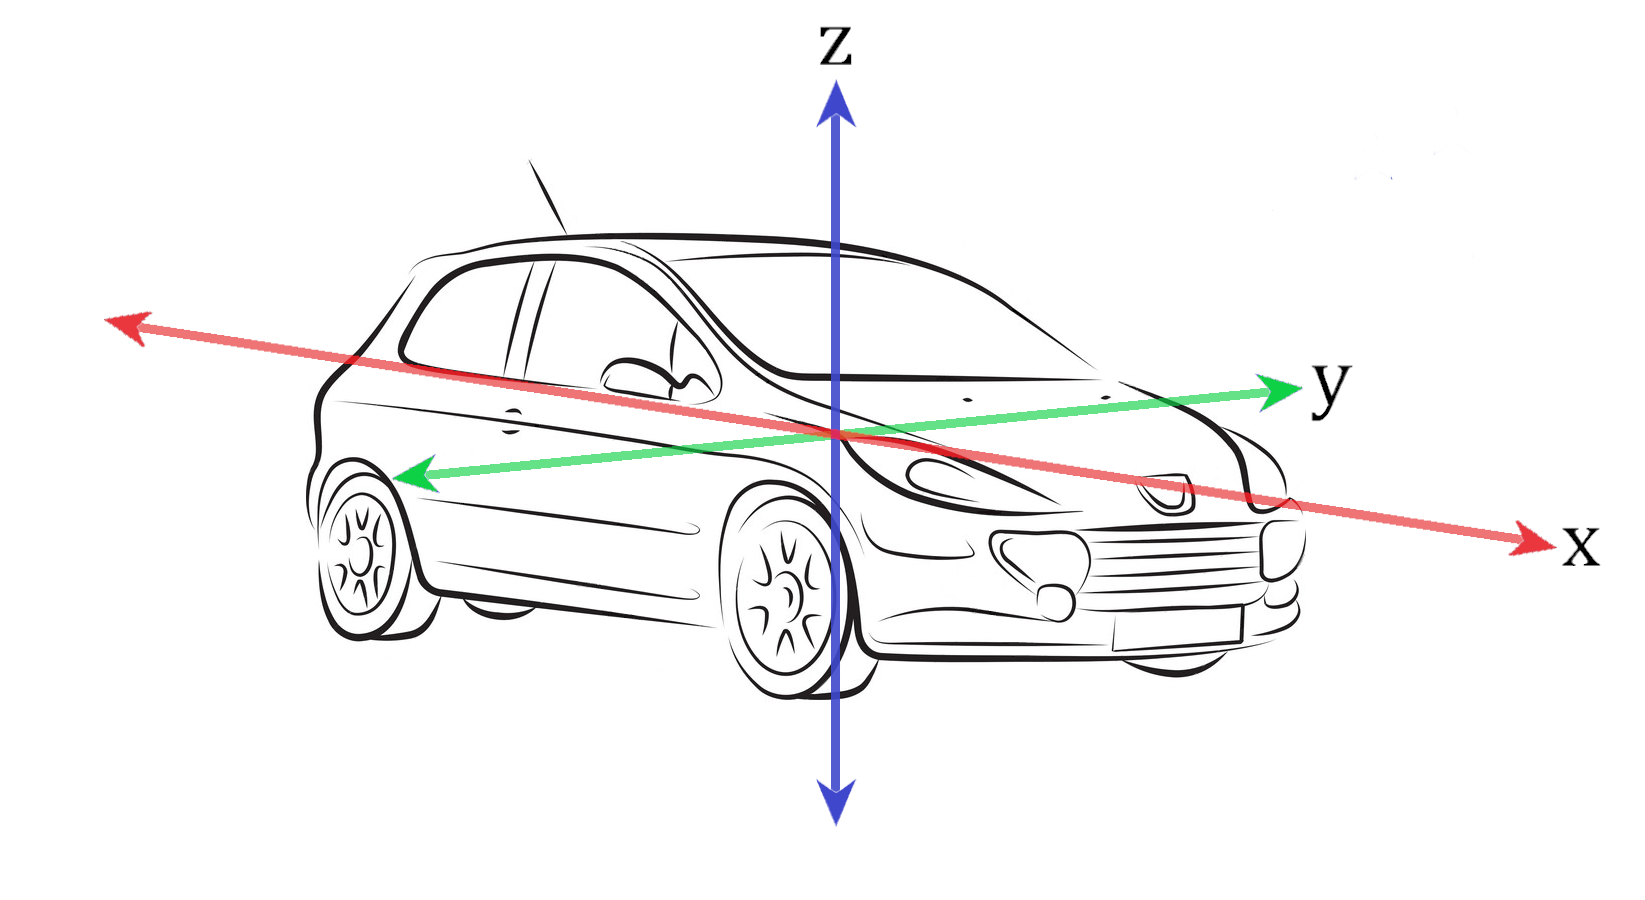
\includegraphics[scale=0.3]{car9.png}
\end{figure}
\end{textblock*}
\end{frame}



\begin{frame}{}
\graficaespectros{Espectro_fxs.pdf}{Frenado}{x}{0.8cm}{Frecuencias características}
\end{frame}



\begin{frame}{}
\graficaespectros{Espectro_rxs.pdf}{Rebase}{y}{0.8cm}{Frecuencias características}  
\end{frame}



\begin{frame}{}
\graficaespectros{Espectro_zyc.pdf}{Movimiento en zig-zag}{y}{0.8cm}{\hskip 5pt Frecuencia característica}
\end{frame}



\begin{frame}{}
\graficaceroeventos{2x.pdf}{Conducción regular}{x}{0.8cm}
\end{frame}



\begin{frame}{}
\graficaceroeventos{2y.pdf}{Conducción regular}{y}{0.8cm}
\end{frame}



\begin{frame}{}
\graficaceroeventos{2z.pdf}{Conducción regular}{z}{0.8cm}
\end{frame}



\begin{frame}{}
\graficauneventos{4y.pdf}{\hskip 3pt Rebase}{y}{0.8cm}
\end{frame}



\begin{frame}{}
\graficauneventos{4z.pdf}{\hskip 3pt Rebase}{z}{0.8cm}
\end{frame}



\begin{frame}{}
\graficadoseventos{5x.pdf}{Movimiento en zig-zag}{\hskip 2pt Rebase}{x}{0.8cm}
\end{frame}



\begin{frame}{}
\graficadoseventos{5z.pdf}{Movimiento en zig-zag}{\hskip 2pt Rebase}{z}{0.8cm}
\end{frame}



\begin{frame}{}
\graficatreseventos{6z.pdf}{Recorrido para validación}{\hskip 2pt Zig-zag}{Frenado}{\hskip 2pt Rebase}{z}{0.8cm}
\end{frame}



\begin{frame}{}
\graficadeteccion{Deteccion_3_C.pdf}{de frenado (cosenos)}{}{\hskip 1pt Regular}{\hskip 2pt Rebase}{\hskip 2pt Zig-zag}{Frenado}{0.8cm}
\end{frame}



\begin{frame}{}
\graficadeteccion{Deteccion_3_S.pdf}{de frenado (senos)}{}{\hskip 2pt Rebase}{Regular}{\hskip 2pt Zig-zag}{Frenado}{0.8cm}
\end{frame}



\begin{frame}{}
\graficadeteccion{Deteccion_4_C.pdf}{de rebase (cosenos)}{}{\hskip 2pt Rebase}{Regular}{}{}{0.8cm}
\end{frame}



\begin{frame}{}
\graficadeteccion{Deteccion_4_S.pdf}{de rebase (senos)}{}{\hskip 2pt Rebase}{Regular}{Zig-zag}{}{0.8cm}
\end{frame}



\begin{frame}{}
\graficadeteccion{Deteccion_5_C.pdf}{de movimiento en zig-zag (cosenos)\vspace{0.5cm}}{}{\hskip 2pt Rebase}{Regular}{\hskip 2pt Zig-zag}{}{0.8cm}
\end{frame}



\begin{frame}{}
\graficadeteccion{Deteccion_5_S.pdf}{de movimiento en zig-zag (senos)\vspace{0.5cm}}{}{\hskip 2pt Rebase}{Regular}{\hskip 2pt Zig-zag}{}{0.8cm}
\end{frame}



\begin{frame}{}
\graficadeteccion{Deteccion_6_C.pdf}{para validación (cosenos)}{}{Regular}{\hskip 2pt Zig-zag}{\hskip 2pt Rebase}{Frenado}{0.8cm}
\end{frame}



\begin{frame}{}
\graficadeteccion{Deteccion_6_S.pdf}{para validación (senos)}{}{\hskip 2pt Rebase}{Regular}{\hskip 2pt Zig-zag}{\hskip -1pt Frenado}{0.8cm}
\end{frame}



\begin{frame}{}
\graficadeteccion{Deteccion_6_CxS.pdf}{para validación  (producto de salidas)\vspace{0.5cm}}{}{Regular}{Zig-zag}{Rebase}{\hskip -1pt Frenado}{0.8cm}
\end{frame}



\begin{frame}{}
\graficasalidas{Salidas_3_C.pdf}{de frenado  (cosenos)}{Componente 1}{Componente 2}{Componente 3}{}{0.8cm}
\end{frame}



\begin{frame}{}
\graficasalidas{Salidas_3_S.pdf}{de frenado (senos)}{Componente 1}{Componente 2}{Componente 3}{}{0.8cm}
\end{frame}



\begin{frame}{}
\graficasalidas{Salidas_4_C.pdf}{de rebase (cosenos)}{Componente 1}{Componente 2}{Componente 3}{}{0.8cm}
\end{frame}



\begin{frame}{}
\graficasalidas{Salidas_4_S.pdf}{de rebase (senos)}{Componente 1}{Componente 2}{Componente 3}{}{0.8cm}
\end{frame}



\begin{frame}{}
\graficasalidas{Salidas_5_C.pdf}{de movimiento en zig-zag (cosenos)\vspace{0.5cm}}{Componente 1}{Componente 2}{Componente 3}{}{0.8cm}
\end{frame}



\begin{frame}{}
\graficasalidas{Salidas_5_S.pdf}{de movimiento en zig-zag (senos)\vspace{0.5cm}}{Componente 1}{Componente 2}{Componente 3}{}{0.8cm}
\end{frame}



\begin{frame}{}
\graficasalidas{Salidas_6_C.pdf}{para validación (cosenos)}{Componente 1}{Componente 2}{Componente 3}{}{0.8cm}
\end{frame}



\begin{frame}{}
\graficasalidas{Salidas_6_S.pdf}{para validación (senos)}{Componente 1}{Componente 2}{Componente 3}{}{0.8cm}
\end{frame}



\begin{frame}{}
\graficasalidas{Salidas_6_CxS.pdf}{para validación (producto de salidas)\vspace{0.5cm}}{Componente 1}{Componente 2}{Componente 3}{}{0.8cm}
\end{frame}



\end{document}
